\documentclass{curs}

% Comment out lines below in case of no code to be included.
%\usepackage{code/highlight}
\usepackage{color}
\usepackage{graphicx}
\usepackage{listings}
\usepackage{multicol}
%\usepackage{alltt}


\title[Session 11]{Session 11}
\subtitle{Software Verification}
\author{Security of Information Systems (SIS)}
\date{January 11, 2019}

\begin{document}

\frame{\titlepage}

\section{Software Verification}

% 1. Plecat de la noțiunile din cursul Lorinei: testarea sistemelor de
% calcul, auditarea lor (caz particular: auditarea codului), inspectarea
% implementării, ce avantaje și dezavantaje are fiecare metodă;
% 
% 2. Introducerea ideii de garanție matematică de corectitudine/securitate
% și ce garanții pot fi oferite mai exact: garantarea unor proprietăți ale
% design-ului (de exemplu garanții pe care le oferă un protocol; sau
% garanții pe care le oferă o primitivă de cripto); proprietăți la nivelul
% limbajului (de exemplu exploit-urile pornesc de la faptul că mașinile de
% calcul expun pointerii programatorului; altfel limbajele memory safe au
% apărut odată cu primele calculatoare); proprietăți ale algoritmului
% versus proprietăți ale implementării; nu îmi e clar cum ar trebui
% prezentată partea asta, dar mi se pare fundamentală pentru a înțelege ce
% înseamnă de fapt verificare formală;
% 
% 3. Recapitulare a problemelor din fundamentele matematicii și științei
% calculatoarelor (Russel, Gödel, halting problem); aici clar materialul e
% super-greoi, dar aș pleca de la ideea că matematica nu poate demonstra
% chiar orice și aș lua mai încolo câteva exemple concrete de ce
% problemele astea ne dau de cap: de exemplu orice componentă
% „continuously running” (serviciu de rețea, nucleul sistemului de
% operare) nu se termină, fapt ce îi face viața grea matematicianului.
% 
% 4. Exemplu de jucărie (probabil ar merge chiar mai devreme) de formal
% proof; nu îmi dau seama ce ar merge mai bine aici, probabil un algoritm
% simplu (însumarea elementelor unui array) sau o chestie mai real-life,
% gen modelarea politicilor de trafic aerian dintr-un aeroport; sau și mai
% bine, ceva pe scurt despre politicile de securitate din iOS (ceva care
% poate fi reprezentat ușor cu conectori logici);
% 
% 5. Motivarea metodelor formale/exemple de verificare formală în systems:
% aici aș pleca de la necesitatea în sisteme critice (avioane, centrale
% nucleare) și aș extinde apoi spre securitate; ideea e că vrei ca
% (a). sistemul să eșueze determinist (să poți avea un grad de control
% asupra fiabilității) și (b). să se comporte determinst; securitatea (în
% particular cea software) ține mai mult de (b) decât de (a), deși (a) e
% important e.g. pentru apărarea împotriva denial of service (atacatorul
% poate să vrea pur și simplu să facă disable la infrastructura critică);
% 
% 6. Ideea de model de atac (nu îmi e clar dacă nu trebuie prezentată
% chiar mai devreme): ce vrea să obțină atacatorul, care e suprafața de
% atac, ce presupuneri putem face; asta se întoarce oarecum la discuția
% legată de „algoritm versus implementare”, pentru că verificarea
% implementărilor în general face multe presupuneri (e.g. legate de
% hardware și compilator).

% Alin: De prezentat Meltdown și Specter din punctul de vedere al verificării formale:
% https://webkit.org/blog/8048/what-spectre-and-meltdown-mean-for-webkit/
% https://lwn.net/Articles/742702/

%O idee care o am eu, daca tot plecati de la testare, ar fi sa vorbiti de faptul ca este un intreg spectru intre testare si verificare formala, in ceea ce a inceput sa se numeasca Runtime Verification.  Si aici sunt niste lucruri care sunt mai usor de inghitit de studenti, cum ar fi
%monitorizarea, eventual cu cod de recovery, care din cate stiu eu e folosita in securitate.
%
%chestia faina cu monitorizarea e ca merge bine in orice situatie, si de multe ori  nici nu mai trebuie sa demonstrezi corectitudinea completa, daca ai instrumentare buna si cod de recovery.
%
%apoi, pentru verificare, puteti vorbi despre
%* (symbolic) model checking, care e muult mai folosit in verificarea hardware, dar are ceva popularitate si in software.  Exemplu clasic, cu tutoriale si toy examples SPIN (si Promela) folosind LTL
%* lighweight verification folosind type systems, si, in general abstract interpretations, in care interpretezi programul intr-un domeniu redus, pentru a obtine niste garantii gen absenta dereferentierii de null pointers, tainting analysis, etc.
%* full program verification, unde folosesti Hoare Logic sau chestii mai avansate ca sa construiesti weakest precondition pentru ca un program sa ajunga in starea finala satisfacand ceva, sau strongest postcondition la care se poate ajunge dintr-o stare initiala data.  Din pacate full program verification merge
%
%Acum, toate astea pot avea aplicatii in securitate.  Provable security probabil poti obtine doar din symbolic model checking sau full program verification.  si probabil doar daca codul tau e impartit in bucatele mici pe care le poti analiza separat.

\begin{frame}{Securing Software}
  \begin{itemize}
    \item verification
    \item code analysis
    \item fuzzing
    \item testing
    \item monitoring
  \end{itemize}
\end{frame}

\begin{frame}{Software Verification}
  \begin{itemize}
    \item before/during implementation
    \item system model/specification
    \item security properties
    \item formal verification
  \end{itemize}
\end{frame}

\begin{frame}{Software Verification}
  \begin{figure}
    \centering
    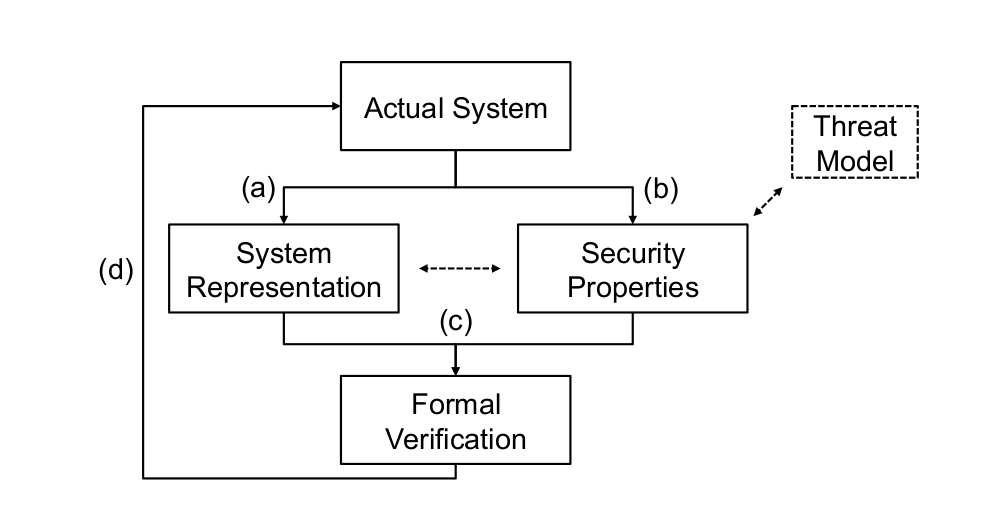
\includegraphics[width=0.7\textwidth]{img/software-verification-procedure} \\
    {\tiny Survey of Approaches for Security Verification of Hardware/Software Systems}
  \end{figure}
\end{frame}

\begin{frame}{System Representation}
  \begin{itemize}
    \item HDL (for hardware)
    \item high-level programming languages
    \item system model
    \item difficult to prove equivalance between system model and the actual system (i.e. implementation)
  \end{itemize}
\end{frame}

\begin{frame}{Security Properties}
  \begin{itemize}
    \item confidentiality, integrity, availability
    \item non-interference
    \item isolation
    \item information flow
    \item type and memory safety
    \item memory integrity
    \item code integrity
  \end{itemize}
\end{frame}

\begin{frame}{Algorithm vs Implementation}
  \begin{itemize}
    \item algorithm verification is mostly theoretical / formal
    \item implementation is particular to the environment: programming language, operating system, hardware
    \item out-of-algorithm components need to be considered when evaluating implementation
  \end{itemize}
\end{frame}

\begin{frame}{Runtime Verification}
  \begin{itemize}
    \item monitoring
    \item detecting and correcting malfunction
    \item recovery code/functions
  \end{itemize}
\end{frame}

\section{Formal Verification}

\begin{frame}{Deductive vs Algorithmic Mechanisms}
  \begin{itemize}
    \item deductive: logical formulas limiting system states throughout execution, relations between states
    \item algorithmic: invariants in the system, i.e. values, variables that are valid among all execution paths
  \end{itemize}
\end{frame}

\begin{frame}{Formal Verification via Deductive Mechanisms}
  \begin{itemize}
    \item general property verification
      \begin{itemize}
        \item deduce properties from system model
        \item represent properties in a theorem prover
        \item prove system S fits a given property P
        \item any system represented as S can be verified against that property P
      \end{itemize}
    \item individual verification
      \begin{itemize}
        \item verify each system
        \item no need to formally define a security property as P
        \item method is not general
      \end{itemize}
    \item Coq, Isabelle, pen-and-paper
  \end{itemize}
\end{frame}

\begin{frame}{Formal Verification via Algorithmic Mechanisms}
  \begin{itemize}
    \item done on system representation and states
    \item model checkers, SMT solvers, symbolic execution
  \end{itemize}
\end{frame}

\begin{frame}{Model Checking}
  \begin{itemize}
    \item given a finite-state model, check that a property holds
    \item define property as a logical formula
    \item do checks using invariants, pre-conditions and post-conditions
    \item state explosion
    \item SPIN (PROMELA)
  \end{itemize}
\end{frame}

\begin{frame}{SMT Solvers}
  \begin{itemize}
    \item Satisfiability Modulo Theories
    \item translate systems into logical formulas
    \item SMT formula validates a property against translated logical formulas
    \item Z3, Boogie
  \end{itemize}
\end{frame}

\begin{frame}{Symbolic Execution}
  \begin{itemize}
    \item symbols used instead of actual values
    \item simulate execution
    \item path explosion
  \end{itemize}
\end{frame}

\begin{frame}{Limitations}
  \begin{itemize}
    \item completeness: what properties do we want to verify
    \item design/algorithm vs implementation
    \item system complexity
  \end{itemize}
\end{frame}

\section{Summary}

\begin{frame}{Keywords}
  \begin{columns}
    \begin{column}{0.5\textwidth}
      \begin{itemize}
        \item TODO
      \end{itemize}
    \end{column}
    \begin{column}{0.5\textwidth}
      \begin{itemize}
        \item TODO
      \end{itemize}
    \end{column}
  \end{columns}
\end{frame}

\begin{frame}{Resources}
  \begin{itemize}
    \item TODO
  \end{itemize}
\end{frame}

\begin{frame}{References}
  \begin{itemize}
    \item TODO
  \end{itemize}
\end{frame}

\end{document}
